\documentclass[10pt, a4paper, spanish]{article}  	% use "amsart" instead of "article" for AMSLaTeX format
\usepackage{geometry}                		% See geometry.pdf to learn the layout options. There are lots.
\geometry{letterpaper}                   		% ... or a4paper or a5paper or ... 
%\geometry{landscape}                		% Activate for rotated page geometry
%\usepackage[parfill]{parskip}    		% Activate to begin paragraphs with an empty line rather than an indent
\usepackage[spanish, es-noindentfirst]{babel}
\selectlanguage{spanish}
\usepackage[utf8]{inputenc}
\usepackage{graphicx}				% Use pdf, png, jpg, or eps§ with pdflatex; use eps in DVI mode
								% TeX will automatically convert eps --> pdf in pdflatex		
\usepackage{amssymb}
\usepackage{array}
%SetFonts

%SetFonts


\title{Visión por computador - Laboratorio 4}
\author{Johnny Torres}
%\date{}							% Activate to display a given date or no date

\begin{document}
\maketitle
\section{Ejercicio 1}
\subsection{Que es el parámetro SIGNAL to NOISE RATIO y como se calcula?}
Se refiere al radio de la señal  a ruido en decibeles de una señal x, al calcular el radio de la suma de la señal al cuadrado con respecto a la señal de ruido y.

\subsection{Generar versiones de Lenna en escala de gris con tres tipos de ruido.}

\begin{table}[h!]
\caption{SNR}
\begin{tabular}{|c|c|c|}
\hline
Tipo Imagen & Imagen & SNR \\
\hline
Original & 	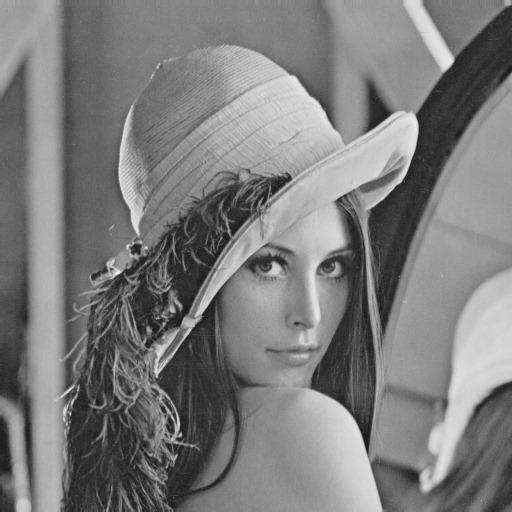
\includegraphics[width=0.25\linewidth]{lenaGray} & \\ 
\hline
Ruido Tipo Gausiano & 	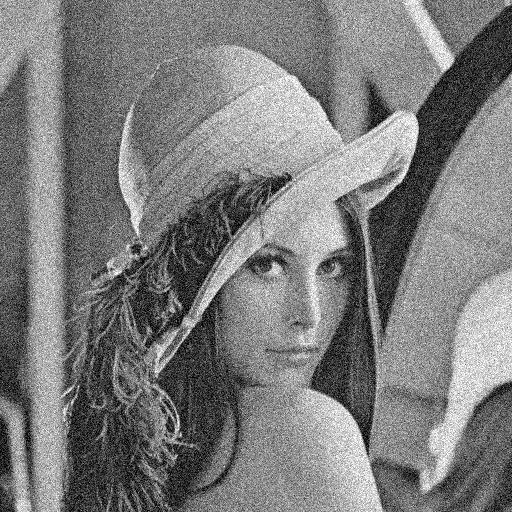
\includegraphics[width=0.25\linewidth]{lenaNoiseGaussian} & 14.4156 \\
\hline
Ruido Tipo Poisson & 	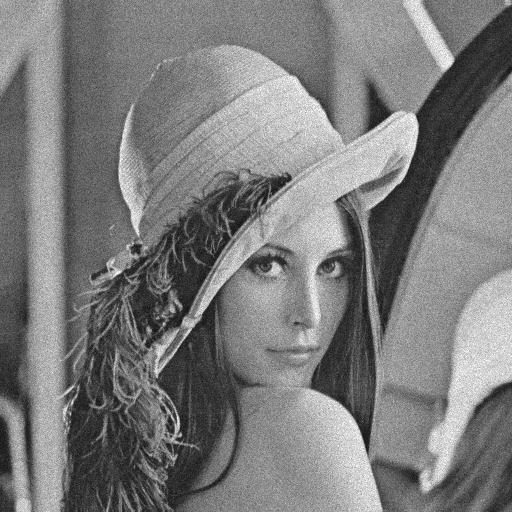
\includegraphics[width=0.25\linewidth]{lenaNoisePoisson} & 21.5386\\
\hline
Ruido Tipo Salt-Pepper & 	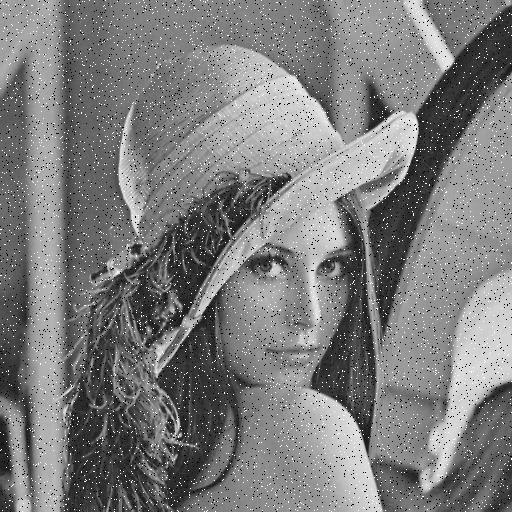
\includegraphics[width=0.25\linewidth]{lenaNoiseSP} & 18.4281\\

\hline
\end{tabular}
\label{default}
\end{table}

\begin{table}[h!]
\caption{SNR con filtros}
\begin{tabular}{|c|c|c|}
\hline
Tipo Imagen & Imagen & SNR \\
\hline
Original & 	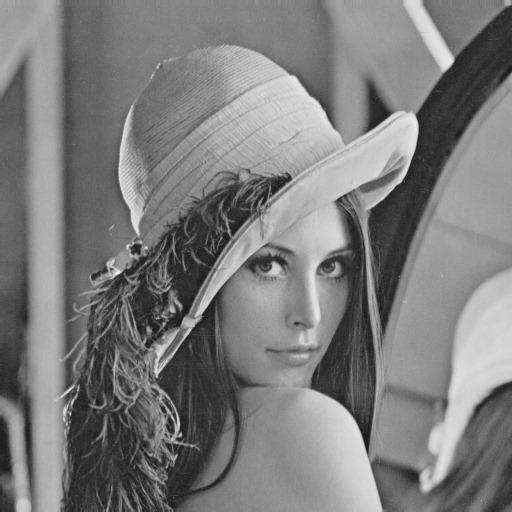
\includegraphics[width=0.25\linewidth]{lenaGray} & \\ 
\hline
Filtro Gaussian & 	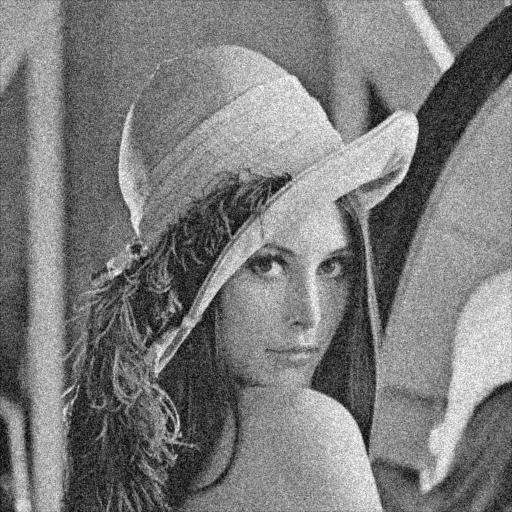
\includegraphics[width=0.25\linewidth]{lenaNoiseGaussianF} & 18.1814\\
\hline
Filtro Unsharp & 	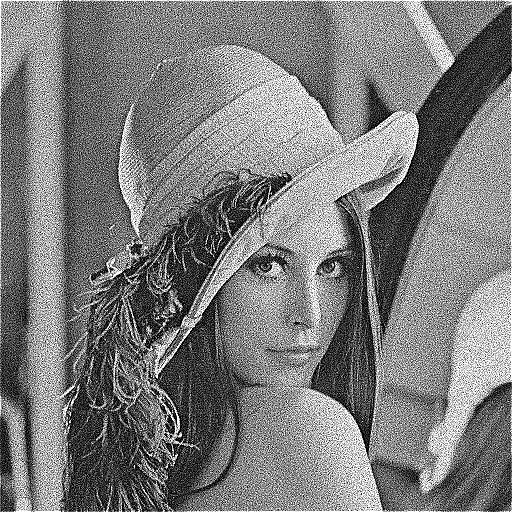
\includegraphics[width=0.25\linewidth]{lenaNoisePoissonF} & 21.5381\\
\hline
Filtro Median & 	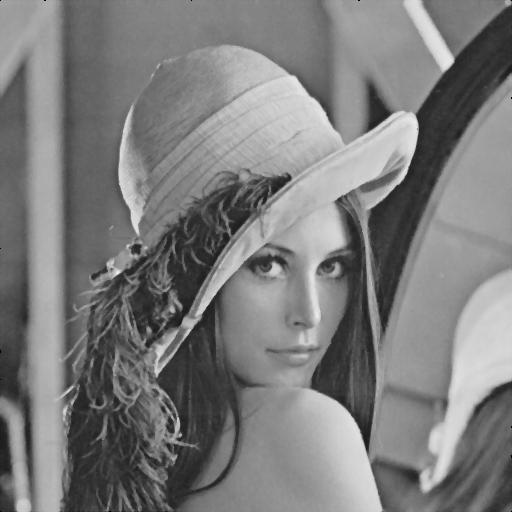
\includegraphics[width=0.25\linewidth]{lenaNoiseSPF} & 28.7371\\

\hline
\end{tabular}
\label{default}
\end{table}

El mejor resultado se consigue luego de aplicar filtro median a la imagen con ruido Salt-Pepper con un SNR 28.7

\clearpage
\section{Ejercicio 2}

\subsection{Filtrado del dominio frecuencial}
El mejor resultado en los experimentos se obtuvo de usar los filtros F'= sobel y F''=gaussian con alpha 0.1
\begin{table}[h!]
\caption{Filtrado frecuencial}
\begin{tabular}{|c|c|c|}
\hline
Filtro & Imagen & Alpha \\
\hline
Sobel/Gaussian & 	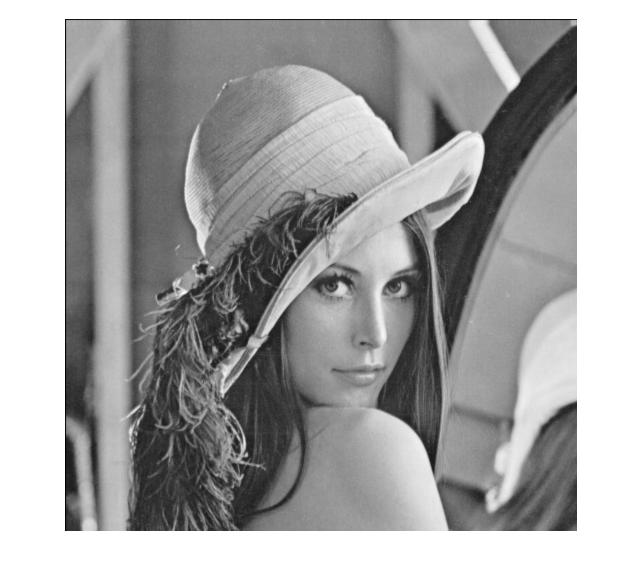
\includegraphics[width=0.25\linewidth]{lenaFreq1} & 0.01\\ 
\hline
Sobel/Gaussian & 	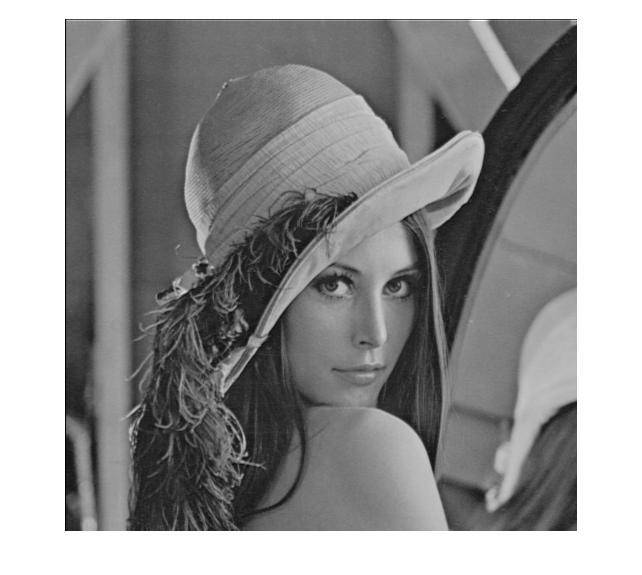
\includegraphics[width=0.25\linewidth]{lenaFreq2} & 0.1 \\
\hline
Sobel/Gaussian & 	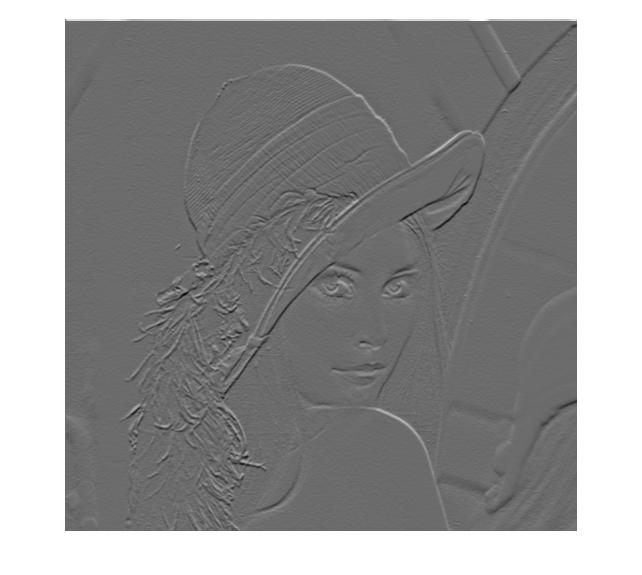
\includegraphics[width=0.25\linewidth]{lenaFreq3} & 1\\
\hline
\end{tabular}
\label{default}
\end{table}


\end{document}  